\documentclass[12pt]{report}
\usepackage{geometry}
\usepackage{titlesec}

\geometry{
a4paper,
left=38mm,
top=25mm,
bottom=25mm,
right=25mm
}
\usepackage{sectsty}
\usepackage{graphicx}
\usepackage{amssymb}
\usepackage{commath}
\usepackage{float}
\usepackage[ruled,vlined]{algorithm2e}
\usepackage{setspace}

\chaptertitlefont{\Large}

\newcommand{\argmin}[1]{\underset{#1}{\operatorname{arg}\,\operatorname{min}}\;}
\newgeometry{top=0.5in,bottom=0.5in,right=1in,left=1in}
\title{
{\fontsize{18}{12}{\textbf{COLLISION AVOIDANCE AND FORMATION CONTROL FOR MULTI-AGENT SYSTEMS}}}\\
\vspace{40pt}
{\normalsize {A thesis submitted in partial fulfillment of the requirements for the award of the degree of}\\
\vspace{12pt}
{\textbf{B.Tech}}\\
\vspace{12pt}
{\textbf{in}}}\\
{\fontsize{14}{12}\textbf{Instrumentation and Control Engineering}}\\
\vspace{12pt}
\onehalfspacing
{\normalsize By}\\
{\fontsize{14}{12} \textbf{Rishab Balasubramanian - 110116070\\
Lalita Soundari - 110116046}}\\
\singlespacing
\vspace{12pt}

\includegraphics[scale=0.15]{NITT_logo.png}\\
\vspace{12pt}
{\textbf{\fontsize{16}{20}{Department of Instrumentation And Control Engineering\\
National Institute of Technology\\
Tiruchirapalli - 620015}}}
\date{June 2020}
}

\usepackage{biblatex}
\addbibresource{refs.bib}

\begin{document}
\maketitle
\newgeometry{
a4paper,
left=38mm,
top=25mm,
bottom=25mm,
right=25mm
}
\onehalfspacing
\newpage

\begin{center}
\textbf{\large{BONAFIDE CERTIFICATE}}
\end{center}

\vspace{25mm}

This is to certify that the project titled \textbf{COLLISION AVOIDANCE AND FORMATION CONTROL FOR MULTI-AGENT SYSTEMS} is a bonafide record of the work done by
\vspace{15mm}

\begin{center}
\textbf{Rishab Balasubramanian - 110116070\\
Lalita Soundari - 110116046}
\end{center}
\vspace{15mm}

in partial fulfillment of the requirements for the award of the degree of \textbf{Bachelor of Technology} in \textbf{Instrumentation And Control Engineering} of the \textbf{NATIONAL INSTITUTE OF TECHNOLOGY, TIRUCHIRAPPALLI}, during the year 2019-2020.

\vspace{15mm}
\begin{flushleft}
\hspace{5mm}\textbf{Dr. M. Umapathy \hspace{70mm} Dr. G. Uma}\\
\hspace{15mm}Guide \hfill Head of the Department
\end{flushleft}
\vspace{15mm}

\begin{flushleft}
Project Viva-Voce held on \rule{100mm}{0.2mm}
\end{flushleft}

\vspace{15mm}

\begin{flushleft}
\hspace{5mm}\textbf{Internal Examiner \hspace{60mm} External Examiner}
\end{flushleft}


\fontsize{12}{18}
\newpage
\chapter*{1.  Abstract}
\addcontentsline{toc}{chapter}{\numberline{1}Abstract}

In this work, we present a formal approach to reciprocal n-body collision
avoidance, where multiple mobile robots need to avoid collisions with each other
while moving in a common workspace. In the formulation presented, each robot acts fully independently, and does not communicate with other robots. Based on the definition
of velocity obstacles, we derive sufficient conditions for collision-free motion
by reducing the problem to solving a low-dimensional linear program. The algorithm is based upon the Optimal Reciprocal Collision Avoidance (ORCA). We test our approach in simulation scenarios and compute collision-free actions for all of them in only a few milliseconds, using software-in-the-loop Gazebo ROS simulatior.

\vspace{10mm}

\begin{flushleft}
\textit{Keywords: }Multi-agent, collision avoidance, robot, ORCA, reciprocal velocity, reciprocal colision avoidance, optimization
\end{flushleft}

\newpage
\chapter*{2.  Acknowlwdgements}

We wish to express our sincere thanks to our research guide, Dr. M. Umapathy, for
providing us with all the expertise and knowledge for the implementation of our
project work and for having faith in our aptitude through this entire period. We would
also like to extend our gratitude to all the faculty and staff members of the department
of Instrumentation and Control Engineering for their support and guidance.



\addcontentsline{toc}{chapter}{\numberline{2}Acknowldegements}
\tableofcontents
\begin{center}
\chapter*{3.  List of Figures}
\addcontentsline{toc}{chapter}{\numberline{3}List of Figures}
\end{center}

\begin{center}
\chapter*{4.  Introduction}
\addcontentsline{toc}{chapter}{\numberline{4}Introduction}
\end{center}

\setcounter{chapter}{4}
\section{Multi-Agent Systems}
A multi-agent system (MAS or ``self-organized system") is a computerized system composed of multiple interacting intelligent agents. Multi-agent systems can solve problems that are difficult or impossible for an individual agent or a monolithic system to solve. 
Multi-agent systems consist of agents and their environment. Typically multi-agent systems research refers to software agents. However, the agents in a multi-agent system could equally well be robots, humans or human teams. A multi-agent system may contain combined human-agent teams. Agents can be divided into types spanning simple to complex. Categories include:

		1.Passive agents or "agent without goals" (such as obstacle, apple or key in any simple simulation)
		
    	2.Active agents with simple goals (like birds in flocking, or wolf–sheep in prey-predator model)\\
    	
Agent environments are split in two: Discrete and Continuous. Agent environments can also be organized according to properties such as accessibility (whether it is possible to gather complete information about the environment), determinism (whether an action causes a definite effect), dynamics (how many entities influence the environment in the moment), discreteness (whether the number of possible actions in the environment is finite), episodicity (whether agent actions in certain time periods influence other periods), and dimensionality (whether spatial characteristics are important factors of the environment and the agent considers space in its decision making). Agent actions are typically mediated via an appropriate middleware. This middleware offers a first-class design abstraction for multi-agent systems, providing means to govern resource access and agent coordination.

\newpage
\section{Collision Avoidance \& Formation Control}

Collision avoidance is a fundamental problem in robotics. The problem can gen-
erally be defined in the context of an autonomous mobile robot navigating in an
environment with obstacles and/or other moving entities, where the robot employs a
continuous cycle of sensing and acting. In each cycle, an action for the robot must be
computed based on local observations of the environment, such that the robot stays
free of collisions with the obstacles and the other moving entities, while making
progress towards a goal. Note that the problem of (local) collision-avoidance differs from motion planning, where the global environment of the robot is considered to be known and a complete path towards a goal configuration is planned at once, and collision detection, which simply determines if two geometric objects intersect or not.
The problem of collision avoidance has been well studied for one robot avoiding static or moving obstacles. In this thesis, we address the more involved and less studied problem of reciprocal n-body collision avoidance, where collisions need to be avoided among multiple robots (or any decision-making entities). This problem has important applications in many areas in robotics, such as multi-robot navigation and coordination among swarms of robots. It is also an key component in crowd simulation for computer graphics and VR, modeling of non-player characters in AI, studying flocks of birds and fish in biology, and real-time (air) traffic control. We develop a fast method based on the Optimal Reciprocal Collision Avoidance (ORCA) that simultaneously determines actions for many (possibly thousands of) robots that each may have different objectives. The actions are computed for each robot independently, without communication among the robots or central coordination. Yet, we show that the method guarantees collision-free motion for each of the robots.
We use a simplified robot model, where each robot is assumed to have a sim-
ple shape (circular or convex polygon) moving in a two-dimensional workspace.
Furthermore, we assume that the robot is holonomic, i.e. it can move in any direc-
tion, such that the control input of each robot is simply given by a two-dimensional
velocity vector. Also, we assume that each robot has perfect sensing, and is able
to infer the exact shape, position and velocity of obstacles and other robots in the
environment.
Main results. We use a rigorous approach for reciprocal n-body collision avoidance that provides a sufficient condition for each robot to be collision-free for at least a fixed amount of time into the future, only assuming that the other robots use the same collision-avoidance protocol. Our approach is velocity-based. That implies that each robot takes into account the observed velocity of other robots in order to avoid collisions with them, and also that the robot selects its own velocity from its velocity space in which certain regions are marked as ‘forbidden’ because of the presence of other robots. The formulation infers for each other robot a half-plane (in velocity-space) of velocities that are allowed to be selected in order to guarantee collision avoidance. The robot then selects its optimal velocity from the intersection of all permitted half-planes, which can be done efficiently using linear programming. Under certain conditions with densely packed robots, the resulting linear program may be infeasible, in which case we select the ‘safest possible’ velocity using a three-dimensional linear program.
We experimented with our approach on several complex simulation scenarios
containing thousands of robots. As each robot is independent, we can fully paral-
lellize the computation of the actions for each robot and report very fast real-time
running times. Furthermore, our experiments show that our approach achieves convincing motions that are smooth and collision-free.




Multi-agent Navigation is a field that has recently gained increasing attention both in  the robotics and the control communities, due to the need for autonomous control of more than one mobile robotic agents in the same workspace. While  most  efforts  in  the  past  had  focused  on  centralized  planning, specific real-world applications have  lead researchers throughout the globe to turn their attention to decentralized concepts. Among  the  various  specifications  that  the  control  design  aims  to  impose  on  the  multi-agent  team,  formation convergence and achievement of flocking behavior are two objectives that have been pursued extensively in the last few years. The main feature of  formation control  is the cooperative nature of the equilibria of the system. Agents  must converge to a desired configuration encoded by the inter-agent relative positions.  On the other hand, flocking behavior involves convergence of the velocity vectors and orientations of the agents to a common value at steady state. The main feature of formation control is the cooperative nature of the equilibria of the system. Agents must converge to a desired configuration encoded by the inter-agent relative positions.In  most cases, formation convergence involves kinematic models of the agents’ motion, while  flocking behavior dynamic ones. Hence the problem of flocking motion has rarely been examined in the context of kinematic models of motion. Formation infeasibility is  equivalent to the case when inter-agent objectives cannot occur simultaneously in the state space. By decoupling the two objectives (collision avoidance and formation convergence) it is shown that undercertain assumptions formation infeasibility forces the agents velocity vectors to a common value at steady state.


\begin{center}
\chapter*{5.  Literature Review}
\addcontentsline{toc}{chapter}{\numberline{5}Literature Review}
\end{center}

Collision avoidance is central to many robotics applications,such as multiagent coordination, autonomous navigation through human crowds, pedestrian motion prediction ,and computer crowd simulation. Yet, finding collision-free,time efficient paths around other agents remains challenging,because it may require predicting other agents’ motion andanticipating interaction patterns, through a process that needsto be computationally tractable for real-time implementation. If  there  is  a  reliable  communication network for agents to broadcast their intents (e.g.  goals,  planned  paths),  then collision avoidance can be enforced through a centralized planner. For instance, collision avoidance requirements can be formulated as separation constraints  in an optimization framework for finding a set of jointly feasible and collision-free paths. However, centralized path planning methods can be computationally prohibitive for largeteams. To attain better scalability, researchers have also proposed  distributed  algorithms  based  on  message-passing schemes which resolve local (e.g. pairwise) conflicts without needing to form a joint optimization problem betweenall members of the team. Agents would need to cooperate without necessarily having knowledge of the other agent’s intents.

 Many approaches assume the observed obstacles to be static (i.e. non-moving) [1, 2, 3, 4, 5, 6, 7], and compute an immediate action for the robot that would avert collisions with the obstacle, in many cases taking into account the robot’s kinematics and dynamics. If the obstacles are also moving, such approaches typically repeatedly “replan” based on new readings of the positions of the obstacles. This may work well if the obstacles move slower than the robot, but among fast obstacles (such as crossing a highway), the velocity of the obstacles need to be specifically taken into account. This problem is generally referred to as “asteroid avoidance”, and approaches typically extrapolate the observed velocities in order to estimate the future positions of obstacles [8, 9, 10, 11, 12, 13].
 
The problem of collision avoidance becomes harder when the obstacles are
not simply moving without considering their environment, but are also intelligent
decision-making entities that try to avoid collisions as well. Simply considering
them as moving obstacles may lead to oscillations if the other entity considers all
other robots as moving obstacles as well [14, 15]. Therefore, the reactive nature of
the other entities must be specifically taken into account in order to guarantee that
collisions are avoided. Yet, the robot may not be able to communicate with other
entities and may not know their intents. 

Existing  workon non-communicating collision avoidance can be broadly classified into two categories, reaction-based and trajectory-based.  Reaction-based  methods specify  one-step interaction rules for the current geometric configuration. For example, reciprocal velocity obstacle (RVO) is a reaction-based method that adjusts each  agent’s velocity vector to ensure collision-free navigation. However, since reaction-based methods do not consider evolution of the neighboring agents’ future states, they are short-sighted in time and have been found to create oscillatory and unnatural behaviors in certain situations.In contrast, trajectory-based methods  explicitly account for evolution of the joint (agent and neighbors) future states by  anticipating other agents’ motion. A subclass of non-cooperative approaches propagates the other agents’ dynamics forward in time, and then plans a collision-free path with respect to the other agents’ predicted paths. However, in crowded environments,  the set of predicted paths often marks a large portion of the space untraversable/unsafe, which leads to the freezing robot problem. A key to resolving this issue is to  account for interactions, such that each agent’s motion can affect one another. Thereby, a subclass ofcooperative approaches has been proposed, which first infers the other agents’ intents (e.g. goals), then plans a set of jointly feasible paths for all  neighboring agents in the environment.

Velocity obstacles (VO) [5] have been a successful velocity-based approach to
avoid collisions with moving obstacles; they provide a sufficient and necessary con-
dition for a robot to select velocity that avoids collisions with an obstacle moving at
a known velocity. This approach was extended for robot-robot collision avoidance
with the definition of Reciprocal Velocity Obstacles (RVO), where both
robots were assumed to select a velocity outside the RVO induced by the other robot.
However, this formulation only guarantees collision-avoidance under specific conditions, and does not provide a sufficient condition for collision-avoidance in general. 2 In this paper, we present the principle of optimal reciprocal collision avoidance (ORCA) that overcomes this limitation; ORCA provides a sufficient condition for multiple robots to avoid collisions among one another, and thus can guarantee collision-free navigation.
We note that it is possible to provide a sufficient and necessary condition for
multiple (say n) robots to select collision-avoiding velocities, by defining a composite velocity obstacle in the 2n-dimensional space of velocities of all n robots [1]. However, this is not only computationally impractical, it also requires central coordination among robots. This is incompatible with the type of distributed multi-robot navigation we focus on in this paper, in which each robot independently and simultaneously selects its velocity from its own 2-D velocity space.

Cooperative trajectory-based methods often produce paths with better quality (e.g. shorter time forall  agents to reach their goal) than  that  of reaction-basedmethods. However, planning paths for all other agentsis computationally expensive, and such cooperative approach typically requires more information than is readily available(e.g. other agent’s intended goal). Moreover, due to modelar and measurement uncertainty, the other agents’ actual paths might not conform to the planned/predicted paths, particularly beyond a few seconds into the future. Thus, trajectory-based methods also need to be run at a high (sensor update) rate, which exacerbates the computational problem.The major difficulty in multiagent collision avoidance isthat anticipating evolution of joint states (paths) is desirablebut computationally prohibitive. 



\begin{center}
\chapter*{6.  Problem Definition}
\addcontentsline{toc}{chapter}{\numberline{6}Problem Definition}
\end{center}


In this thesis we work to replicate the results as stated by van den Berg et.al. in their paper "Reciprocal n-Body Collision Avoidance". The problem discussed in the paper, and subsequently in this thesis is formally defined as follows. Let there be a set of n robots sharing an environment. For simplicity, we shall assume that they are restricted to move in the XY- plane of $\mathbb{R}^{2}$.Each robot A has a current position $p_{A}$ (the center of its disc), a current velocity $v_{A}$ and a radius $r_{A}$ . These parameters are part of the robot’s external state, i.e. we assume that they can be observed by other robots. In this thesis we assume that the radius of all robots are equal. Furthermore, each robot has a maximum speed $v_{A}^{max}$, and a preferred velocity $v_{A}^{pref}$. The maximum velocity of the robot is bound by its physical constraints, while we shall define the preferred velocity as the velocity the robot shall assume under the abscence of any obstacles. In this work, we assume the maximum velocities of all robots to be equal.

The task is for each robot A to independently (and simultaneously) select a new
velocity $v_{new}^{A}$ for itself such that all robots are guaranteed to be collision-free for at least a preset amount of time $\tau$ when they would continue to move at their new velocity. As a secondary objective, the robots should select their new velocity as close as possible to their preferred velocity. The robots are not allowed to communicate with each other, and can only use observations of the other robot’s current position and velocity. However, each of the robots may assume that the other robots use the same strategy as itself to select a new velocity.

\begin{center}
\chapter*{7.  Formulation of the Reciprocal Collision Avoidance}
\addcontentsline{toc}{chapter}{\numberline{7}Formulation of the Reciprocal Collision Avoidance}
\end{center}

For two robots A and B, the velocity obstacle $VO^{\tau}_{A|B}$ (called the velocity obstacle of A induced by B in time window $\tau$) is the set of all relative velocities of A with respect to B that will result in a collision between A and B at some moment before time $\tau$. It is formally defined as follows. Let D(p, r) denote an open disc of radius r centered at p;

\begin{equation}
D(p,r) = \{\textbf{q}| \norm{\textbf{q}-p} \leq r\}
\end{equation}

then:
\begin{equation}
VO^{\tau}_{A|B} = \{\textbf{v}|\exists t \in [0,\tau]: t\textbf{v} \in D(p_{A}-p_{A}, r_{A}+r_{B}\} 
\end{equation}
where $p_{B}, r_{B}, p_{A}, r_{A}$ are the positions and radii of A and B respectively.


Let $v_{A}$ and $v_{B}$ be the current velocities of robots A and B, respectively. The 
definition of the velocity obstacle implies that if $v_{A} - v_{B} \in VO^{\tau}_{A|B}$ , or equivalently if $v_{B} - v_{A} \in VO^{\tau}_{B|A}$ , then A and B will collide at some moment before time $\tau$ if they continue moving at their current velocity. Conversely, if $v_{A} - v_{B} \notin VO^{\tau}_{A|B}$ , robot A and B are guaranteed to be collision-free for at least $\tau$ time. 

More generally, let $X \oplus Y$ denote the Minkowski sum of sets X and Y such that
\begin{equation}
X \oplus Y = {x + y | x \in X, y \in Y },
\end{equation}
then for any set $V_{B}$ , if $v_{B} \in V_{B}$ and $v_{A} \notin VO^{\tau}_{A|B} \oplus V_{B}$ , then A and B are guaranteed to be collision-free at their current velocities for at least $\tau$ time. This leads to the definition of the set of collision-avoiding velocities for A given that B selects its velocity from V B (refer Fig. 1(c)):

\begin{equation}
CA^{\tau}_{A|B}(V B ) = {\textbf{v} | \textbf{v} \notin VO^{\tau}_{A|B} \oplus V_{B} }
\end{equation}

We thus call this set $CA^{\tau}_{A|B}$ as the collision avoidance set of velocities for A relative to B. Let us define a vector $u$ as:

\begin{eqnarray}
u = \argmin{v \in \partial VO^{\tau}_{A|B}}(\norm {v-(v_{A}^{opt}-v_{B}^{opt})} - (v_{A}^{opt}-v_{B}^{opt}))\label{eq:dir}
\end{eqnarray}

\begin{figure}[h]
	\centering
	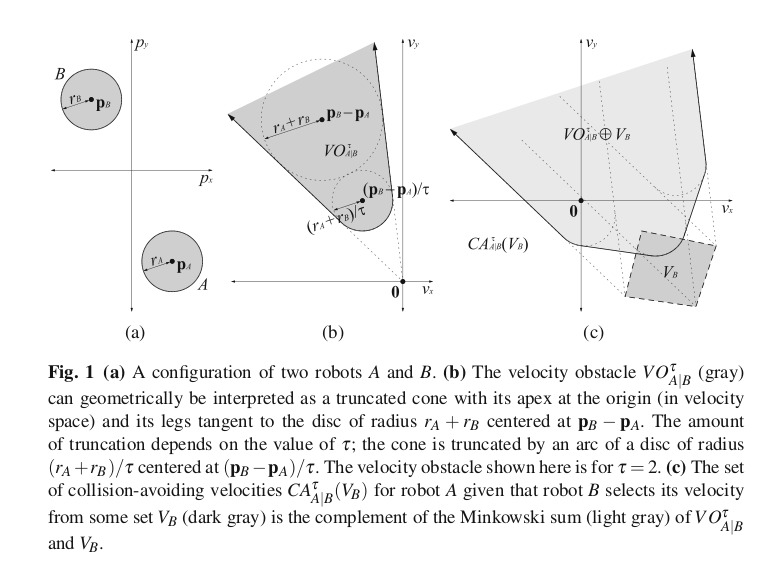
\includegraphics[scale=0.6]{VO.png}  \label{fig:VO}
\end{figure}

\begin{figure}[h]
	\centering
	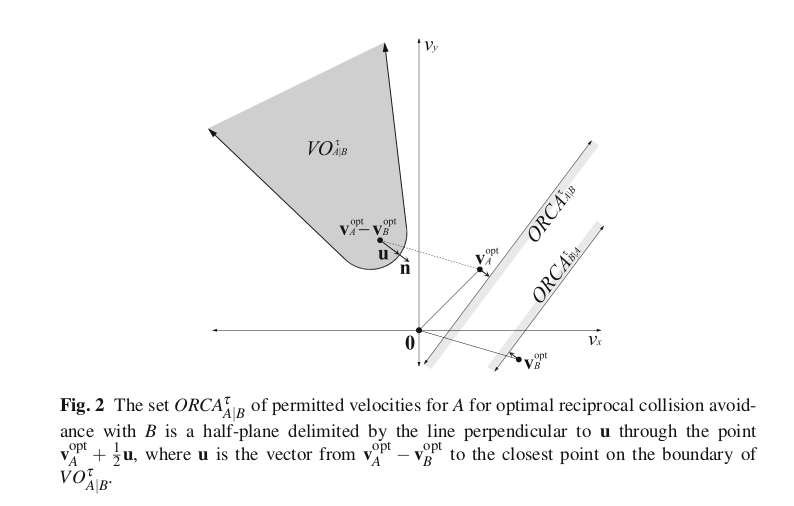
\includegraphics[scale=0.6]{ORCA.png}  \label{fig:ORCA}
\end{figure}

We can see that choosing $v \in \partial VO^{\tau}_{A|B}$ makes $v$ to be a point on the boundary of the velocity obstacle curve formed by A due to B ($VO^{\tau}_{A|B}$). Minimizing Eq.\ref{eq:dir} means that we choose $v$ along $VO^{\tau}_{A|B}$ such that it is closest to the current relative velocity between A and B. We can then construct a hyperplane of collision avoiding velocites, which we shall call $ORCA^{\tau}_{A|B}$ as:

\begin{equation}
ORCA^{\tau}_{A|B} = \{v|(v-(v_{A}^{opt} + \frac{1}{2}u)).n \geq 0\}
\end{equation}\\


This set gives us the hyperplane of collision avoiding velocities. Every velocity in this hyperplane ensures collision avoidance. We select our next velocity $v_{next}$ as:

\begin{equation}
v_{next} = \argmin{v \in ORCA^{\tau}_{A|B}}{\norm {v-v_{A}^{opt}}}
\end{equation}




\chapter*{8.  Applying ORCA to n-robot collision avoidance}
\addcontentsline{toc}{chapter}{\numberline{8}Applying ORCA to n-robot collision avoidance}
\begin{figure}[h]
	\centering
	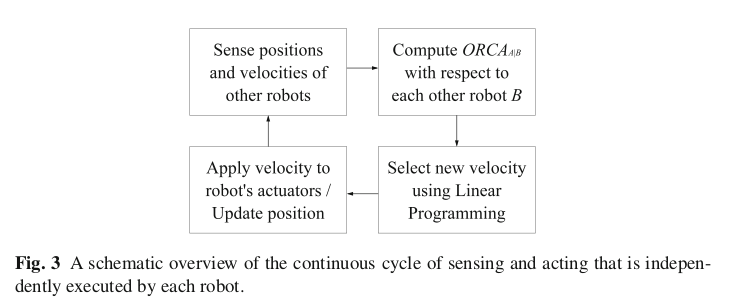
\includegraphics[scale=0.6]{n-body.png}  \label{fig:n-body}
\end{figure}
In this section we shall discuss how to apply the ORCA halfplane segmentation to multiple body systems. Fig.3 shows the basic heirarchy.There are essentially four steps:\\ \\
\begin{algorithm}[h]
\SetAlgoLined
 initialize all robots\;
 \For{each robot}{
	(i) Sense and estimate the position and velocities of other robots, which are in the 		surrounding of robot A and are a velocity obstacle.
	\eIf{robot $B \in VO^{\tau}_{A|B} $}{
  	 Compute the avoidance hyperspace ORCA for robot B with respect to A\;
  	 }{
  	 skip robot B\;
  	 Use Linear programming to select the feasible and ideal velocity\;
  	 New velocity $v_{next}$ is selected as the closest velocity to our preferred velocity $v_{pref}$ according to Eq. \ref{eq:update}\;
  	 Apply the new velocity to and update the new position and velocity \;
  	}
 }
 \caption{Multi body Optimal Reciprocal Collision Avoidance}\label{alg:ORCA}
\end{algorithm}

To obtain the common hyperspace formed by the intersection of all the planes, we use:

\begin{equation}\label{eq:update}
ORCA^{\tau}_{A} = D(0,v^{A}_{max}) \cap \bigcap ORCA^{tau}_{A|B}
\end{equation}

We apply the algorithm as given in Algorithm.\ref{alg:ORCA}. To provide more insight, we shall expand upon the Linear Programming step to select optimal velocities.

\begin{figure}[h]
	\centering
	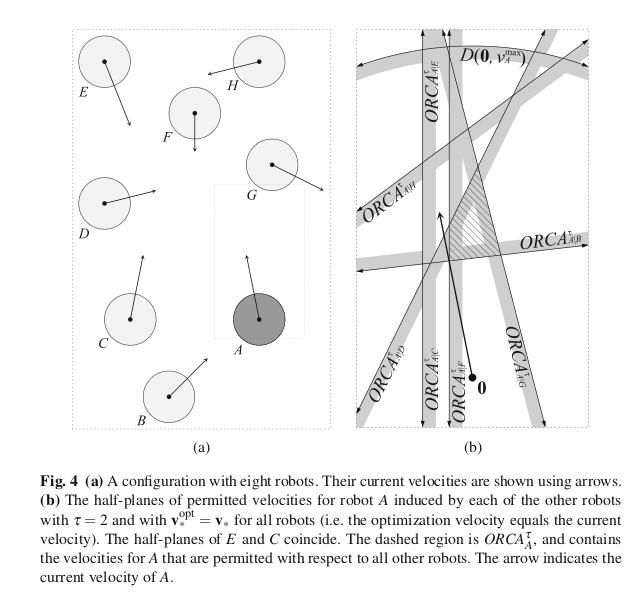
\includegraphics[scale=0.6]{Algo.png}  \label{fig:algo}
\end{figure}

Let us consider a multi-robot situation as in Fig.4. Fig.4(a) shows the various agents and their current velocity. Let us say that all agents act as velocity obstacles to our controlled agent (robot A), and after solving for ORCA between every other robot and robot A, we get various hyperplanes as in Fig.4(b). To find the best feasible solution, we bount all the hyperplanes such that they lie within the circle (sphere in case of 3D situations) or radius $v^{max}_{A}$. Then we find the common region formed by the intersection of these planes, and the point closest to the desired velocity $v^{opt}_{A}$ is our next velocity. We can observe that we shall always have a solution to this optimization problem, simply by observing that by choosing 0 as the next velocity of all robots, we can prevent collision. Therefore, the system of equations is always solvable with a trivial solution in the worst case.




\chapter*{9.  Obtaining Optimal Velocities}
\addcontentsline{toc}{chapter}{\numberline{9}Obtaining Preferred Velocities}

\begin{figure}[h]
	\centering
	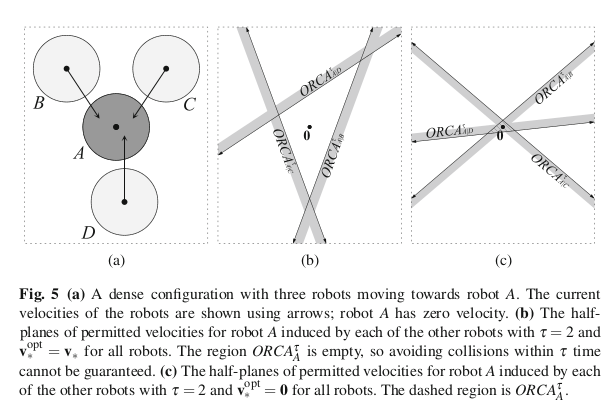
\includegraphics[scale=0.6]{vopt.png}  \label{fig:vopt}
\end{figure}

One issue that we have left open is how to choose the optimal velocity $v^{opt}_{A}$ for each robot A. Here, we discuss some reasonable possibilities:\\
• $v^{opt}_{A}$ = 0 for all robots A. If we set the optimization velocity to zero for all robots, it is guaranteed that $ORCA^{\tau}_{A}$ is non-empty for all robots A (see Fig. 5(c)). Hence, the linear programming algorithm as described above will find a velocity for all robots that guarantees them to be collision-free for at least $\tau$ time. This can be seen as follows. For any other robot B, the point 0 always lies outside the velocity obstacle $VO^{\tau}_{A|B}$ (for finite $\tau$ ). Hence the half-plane $ORCA^{\tau}_{A|B}$ always includes at least velocity 0. In fact, the line delimiting $ORCA^{\tau}_{A|B}$ is perpendicular to the line connecting the current positions of A and B. A drawback of setting the optimization velocity to zero is that the behavior of
the robots is unconvincing, as they only take into account the current positions of
the other robots, and not their current velocities. In densely packed conditions,
this may also lead to a global deadlock, as the chosen velocities for the robots
converge to zero when the robots are very close to one another.\\
• $v^{opt}_{A} = v^{pref}_{A}$ (i.e. the preferred velocity) for all robots A. The preferred velocity is part of the internal state of the robots, so it cannot be observed by the other robots. Let us, for the sake of the discussion, assume that it is somehow possible to infer the preferred velocity of the other robots, and that the optimization
velocity is set to the preferred velocity for all robots. This would work well in low-density conditions, but, as the magnitude of the optimization velocity increases, it is increasingly more likely that the linear program is infeasible. As in most cases the preferred velocity has a constant (large) magnitude, regardless of the density conditions, this would lead to unsafe navigation in even medium density conditions.\\
• $v^{opt}_{A} = v^{cur}_{A}$ (i.e. the current velocity) for all robots A. Setting the optimization to the current velocity is the ideal trade-off between the above two choices, as the current velocity automatically adapts to the situation: it is (very) indicative of the preferred velocity in low-density cases, and is close to zero in dense scenarios. Also, the current velocity can be observed by the other robots. Nevertheless,
the linear program may be infeasible in high-density conditions (see Fig. 5(b)).\\

In this work we used $v^{opt}_{A} = v^{pref}_{A}$. To obtain the preferred velocity for robot A $v^{pref}_{A}$, we apply a PID algorithm. The PID uses the current positions of the robot and its desired goal positions to generate the required velocity commands. To obtain the current robot positions and velocities, we use and IMU atop each agent. We assume that the data is deterministic (not noisy), and hence use this information directly

\chapter*{10.  Simulation Results}
\addcontentsline{toc}{chapter}{\numberline{10}Simulation Results}

\chapter*{11.  Conclusion And Future Work}
\addcontentsline{toc}{chapter}{\numberline{10}Conclusion And Future Work}

We have discussed an efficient method that provides a sufficient condition for multiple robots to select an action that avoids collisions with other robots, though each acts independently without communication with others. The proposed approach to reciprocal n-body collision avoidance exhibits fast running times and smooth, convincing behavior in our experiments. We have used a simple robot model, in which kinematics and dynamics are ignored. An important extension for future work is to take such constraints into ac-
count. We can either do this as a post-processing step, in which the computed new
velocity is ‘clamped’ to what the kinematic and dynamic constraints allow. This
would not strictly guarantee avoiding collisions anymore, but it may work well in
practice. A more thorough solution would be to take these factors intrinsically
into account in the derivation of the permitted velocities for the robots. Also, we have demonstrated results for only 2-D environments. However, all definitions and the algorithm can be extended to 3-D. This may be interesting for applications such as autonomous aerial vehicles, or flocking simulation of birds or fish. Another important direction for future work is to implement the presented framework on real robots and incorporate sensing uncertainty.

\newpage
\addcontentsline{toc}{chapter}{\numberline{}Bibliography}
\begin{thebibliography}{100}
\bibitem{1} Borenstein, J., Koren, Y.: The vector field histogram - fast obstacle avoidance for mobile robots. IEEE Journal of Robotics and Automation 7(3), 278–288 (1991)
\bibitem{2} Faverjon, B., Tournassoud, P.: A local based approach for path planning of manipulators with a high number of degrees of freedom. In: IEEE Int. Conf. Robot. Autom., pp. 1152–1159 (1987)
\bibitem{3} Fox, D., Burgard, W., Thrun, S.: The dynamic window approach to collision avoidance. IEEE Robot. Autom. Mag. 4, 23–33 (1997)
\bibitem{4} Fraichard, T., Asama, H.: Inevitable collision states - a step towards safer robots? Advanced Robotics 18(10), 1001–1024 (2004)
\bibitem{5} Kanehiro, F., Lamiraux, F., Kanoun, O., Yoshida, E., Laumond, J.-P.: A local collision avoidance method for non-strictly convex polyhedra. In: Robotics: Science and Systems (2008)
\bibitem{6} Khatib, O.: Real-Time Obstacle Avoidance for Manipulators and Mobile Robots. Int. Journal of Robotics Research 5(1), 90–98 (1986)
\bibitem{7} Simmons, R.: The curvature-velocity method for local obstacle avoidance. In: IEEE Int.Conf. on Robotics and Automation, pp. 3375–3382 (1996)
\bibitem{8} Fulgenzi, C., Spalanzani, A., Laugier, C.: Dynamic obstacle avoidance in uncertain environment combining PVOs and occupancy grid. In: IEEE Int. Conf. Robot. Autom., pp.1610–1616 (2007)
\bibitem{9} Gil de Lamadrid, J.: Avoidance of Obstacles With Unknown Trajectories: Locally Optimal Paths and Periodic Sensor Readings. Int. Journal of Robotics Research 13(6), 496–507 (1994)
\bibitem{10} Hsu, D., Kindel, R., Latombe, J., Rock, S.: Randomized kinodynamic motion planning with moving obstacles. Int. J. Robot. Res. 21(3), 233–255 (2002)
\bibitem{11} Martinez-Gomez, L., Fraichard, T.: Collision avoidance in dynamic environments: an ICS-based solution and its comparative evaluation. In: IEEE Int. Conf. on Robotics and Automation (2009)
\bibitem{12} Petti, S., Fraichard, T.: Safe motion planning in dynamic environments. In: IEEE RSJ Int. Conf. Intell. Robot. Syst., pp. 2210–2215 (2005)
\bibitem{13} Zucker, M., Kuffner, J., Branicky, M.: Multipartite RRTs for rapid replanning in dynamic environments. In: IEEE Int. Conf. on Robotics and Automation, pp. 1603–1609 (2007)
\bibitem{14} Kluge, B., Prassler, E.: Reflective navigation: Individual behaviors and group behaviors.In: IEEE Int. Conf. Robot. Autom., pp. 4172–4177 (2004)
\bibitem{15} van den Berg, J., Lin, M., Manocha, D.: Reciprocal Velocity Obstacles for real-time multi-agent navigation. In: IEEE Int. Conf. on Robotics and Automation, pp. 1928–1935 (2008)
\bibitem{16} Fiorini, P., Shiller, Z.: Motion planning in dynamic environments using Velocity Obstacles. Int. Journal of Robotics Research 17(7), 760–772 (1998)
\end{thebibliography}

\end{document}